\documentclass[10pt]{beamer}

%\usepackage[french]{babel}
\usepackage{graphicx,color}
\usepackage{subfigure}
\usepackage{listings}
\lstloadlanguages{VHDL,C,XML}
\lstset{frame=none,basicstyle=\tiny,breaklines,tabsize=2,captionpos=b,
prebreak={\hbox{$\rightarrow$}},postbreak={\hbox{$\hookrightarrow$}},
showstringspaces=false,backgroundcolor=\color{grey}\bfseries,
keywordstyle=\color{blue},commentstyle=\color{green}\textit,
stringstyle=\color{red}\ttfamily,abovecaptionskip=2pt,
aboveskip=0pt,belowskip=0pt,belowcaptionskip=0pt}


\setbeamertemplate{background canvas}[vertical
shading][bottom=white,top=structure.fg!25]
\setbeamertemplate{navigation symbols}{}
\usetheme{Hannover}

\beamertemplatefootpagenumber

\definecolor{grey}{rgb}{0.95,0.95,0.95} % on d�finit la couleur grise
\definecolor{red}{rgb}{1.0,0.0,0.0}
\definecolor{green}{rgb}{0.0,0.7.0,0.0}
\definecolor{blue}{rgb}{0.0,0.0,1.0}
\lstloadlanguages{VHDL,C}
\lstset{frame=none,basicstyle=\tiny,breaklines,tabsize=2,captionpos=b,
prebreak={\hbox{$\rightarrow$}},postbreak={\hbox{$\hookrightarrow$}},
showstringspaces=false,backgroundcolor=\color{grey}\bfseries,
keywordstyle=\color{blue},commentstyle=\color{green}\textit,
stringstyle=\color{red}\ttfamily,abovecaptionskip=2pt,
aboveskip=0pt,belowskip=0pt,belowcaptionskip=0pt}

\title[OSCIMP Digital Ecosystem]{
	OSCIMP Digital Ecosystem}
\author[G. GOAVEC-MEROU \& al]{\textbf{Gwenha\"el GOAVEC-MEROU, Jean-Michel
FRIEDT, Pierre-Yves BOURGEOIS}\\ gwenhael.goavec@femto-st.fr\\
IRC \#oscimp channel @ freenode}
\begin{document}
\begin{frame}
\hspace{-0.2cm}\frametitle{Environment for codesign CPU-FPGA}
\vspace{-0.5cm}
\titlepage

\vspace{-0.7cm}
\footnotesize{Slides at \\
\url{www.trabucayre.com/GRDays2019/presentationEcoSystem_GRDays2019.pdf}}

\begin{minipage}[t]{\linewidth}
\begin{minipage}{0.5\linewidth}
\center\includegraphics[width=0.2\textwidth]{./img/plutosdr_github_qrcode.png}\\
\hspace{-0.3cm}\scriptsize{\url{https://github.com/oscimp/PlutoSDR}}
\end{minipage}
\begin{minipage}{0.5\linewidth}
\center\includegraphics[width=0.2\textwidth]{./img/oscimpDigital_github_qrcode.png}\\
\scriptsize{\url{https://github.com/oscimp/oscimpDigital}}
\end{minipage}
\end{minipage}

\end{frame}

\frame{\frametitle{Context}
\begin{minipage}[t]{\linewidth}
\begin{minipage}{0.4\linewidth}
\begin{flushleft}
Redpitaya: dual ADC \& DAC 14bits@125MHz
\end{flushleft}
\end{minipage}
\begin{minipage}{0.55\linewidth}
\begin{flushright}
PlutoSDR: RF Frontend 70~MHz$\to$6~GHz
\end{flushright}
\end{minipage}
\end{minipage}

\vspace{3mm}

$\Rightarrow$ Perfect for acquisition and Digital Signal Processing with codesign CPU/FPGA

FPGA (Real-time) for fast task
\begin{itemize}
\item data acquisition;
\item frequency transposition;
\item filtering;
\item decimation.
\end{itemize}

CPU (General Purpose OS) for slow task after decimation
\begin{itemize}
\item post-processing;
\item display;
\item transmission;
\item configuration
\end{itemize}
}

\frame{\frametitle{Example}
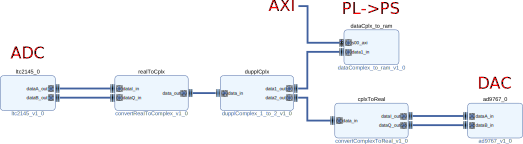
\includegraphics[width=1.0\textwidth]{./img/tutorial3_ann.pdf}

\scalebox{0.31}{
\hspace{-1.5cm}
\input{./pnm_2_ch_noise_floor_setup2.pdf_t}

}

}
%\frame{\frametitle{Example: phase noise}
%\includegraphics[width=1.0\textwidth]{./imgsrc/schema_zc706.pdf}
%
%\vfill
%\tiny{P.-Y. Bourgeois, G. Goavec-Merou, J.-M. Friedt, E. Rubiola :
%A Fully-Digital Realtime SoC FPGA Based Phase Noise Analyzer with
%Cross-Correlation, EFTF-IFCS, Jul 2017.}
%}
%\frame{\frametitle{Example: 2.45~GHz radar}
%
%\includegraphics[width=1.0\textwidth]{./img/schema_design.pdf}
%
%\includegraphics[width=1.0\textwidth]{./img/sortie_affichage_resultat_radar}
%
%\vfill
%\tiny{G. Goavec-Merou, N. Chr\'etien, J.-M Friedt, P. Sandoz, G. Martin, M.
%Lenczner et S. Ballandras : Fast contactless vibrating structure
%characterization using real time field programmable gate array-based digital
%signal processing : Demonstrations with a passive wireless acoustic delay
%line probe and vision. Rev Sci Instrum {\bf 85}(1) :015109 01510910, Jan 2014.}
%
%}
\frame{\frametitle{Consequence}
\vspace{-0.2cm}
\hspace{-0.5cm}
\begin{minipage}[t]{\linewidth}
\begin{minipage}{0.8\linewidth}
\hspace{-0.6cm}
\begin{itemize}
\item one algorithm $\Rightarrow$ one or more flavor (data type, performance vs.
resources, ...): {\tt fpga\_ip} directory
\item need to communicate between FPGA and CPU: {\tt linux\_driver} directory
\item some IPs are widely used or complex to configure $\Rightarrow$ need
to provide library with CPU code (reduce redundance, simplify application): {\tt
liboscimp} in {\tt lib} directory.
\end{itemize}
\end{minipage}
\begin{minipage}{0.1\linewidth}
\center\includegraphics[width=2.6\textwidth]{./img/structureEco}
\end{minipage}
\end{minipage}
}
\frame{\frametitle{OSCIMP EcoSystem}
Purpose~: provide a coherent environment to create design (FPGA), and
application:
\vspace{-0.2cm}
\begin{minipage}[t]{\linewidth}
\begin{minipage}{0.6\linewidth}
\hspace{-0.2cm}
\begin{itemize}
\item blocks (IP) with algorithm level of implementation (FPGA);
\item GNU/Linux hierarchy compliance (driver/library/application);
\item tools to generate some files and scripts/Makefile to factorize most common
part.
\end{itemize}
\end{minipage}
\begin{minipage}{0.3\linewidth}
\center\includegraphics[width=0.7\textwidth]{./img/structureEco}
\end{minipage}
\end{minipage}
\vspace{-0.5cm}
\center\includegraphics[width=1.0\textwidth]{./img/structRepo}
}
%\frame{\frametitle{Structure}
%}
\frame{\frametitle{FPGA}
\begin{minipage}[t]{\linewidth}
\begin{minipage}{0.6\linewidth}
Algorithms or utilities functions.

Developer aspect:
\begin{itemize}
\item normalize interfaces between blocks
\item isolation between implementation and communication
\end{itemize}

End user aspect:
\begin{itemize}
\item 0, 1 or more interface to connect;
\item AXI interface automatically connected.
\end{itemize}
\end{minipage}
\begin{minipage}{0.35\linewidth}
\includegraphics[width=1.2\textwidth]{./img/structureIp}
\end{minipage}
\end{minipage}
\includegraphics[width=0.9\textwidth]{./img/displayIf}
}
\frame{\frametitle{CPU: environment}
{\bf Char device drivers} to add abstraction, GNU/Linux hierarchy compliance and
communication improvement:
\begin{itemize}
\item 1 IP with communication $\Rightarrow$ 1 (or more) driver(s);
\item a {\tt core} driver knows how to communicate with an IP but not where;
\item {\tt device tree overlay} used to provide which drivers must be probed and
base address for each of them;
\end{itemize}
TODO $\Rightarrow$ IIO integration

{\bf libraries} to simplify some common and long (number of line) tasks.
}

\frame{\frametitle{CPU: application}
Application structure:
\begin{itemize}
\item dts to provides which driver must be used and base address;
\item Makefile to cross-compile application and generate the {\tt dtbo} from dts
\item applicationName\_us.sh a shell script used to flash FPGA, load devicetree
and drivers;
\item main.c: user application
\end{itemize}

\includegraphics[width=1.0\textwidth]{img/structApp.pdf}
}

\begin{frame}[containsverbatim]
\frametitle{CPU: module\_generator}
\begin{itemize}
\item Used to generate some files in app directory.
\item use an XML file for design's informations.
\end{itemize}

{\small \verb!module_generator -dts myApp.xml!}

\hspace{-0.6cm}
%\begin{columns}[t]
%\begin{column}{0.57\textwidth}
%myApp.xml
%\vspace{-0.2cm}
{\footnotesize \begin{verbatim}
<?xml version="1.0" encoding="utf-8"?>
<project name="tutorial5" version="1.0">
  <options>
    <option target="makefile" name="USE_STATIC_LIB">1</option>
    <option target="makefile" name="LDFLAGS">-liio</option>
  </options>
  <ips>
    <ip name ="dataComplex_to_ram" >
      <instance name="data1600" id = "0"
        base_addr="0x43c00000" addr_size="0xffff" />
    </ip>
    <ip name ="nco_counter">
      <instance name="nco" id = "0"
        base_addr="0x43c10000" addr_size="0xffff" />
    </ip>
  </ips>
</project>
\end{verbatim}
}

%tutorial5\_us.sh
%\vspace{-0.2cm}
%{\tiny 
%\begin{verbatim}
%cp ../bitstreams/tutorial5_wrapper.bit.bin /lib/firmware
%rmdir /sys/kernel/config/device-tree/overlays/fpga
%mkdir /sys/kernel/config/device-tree/overlays/fpga
%cat tutorial5.dtbo > $DTB_DIR/dtbo
%insmod ../../modules/data_to_ram_core.ko
%insmod ../../modules/nco_counter_core.ko
%\end{verbatim}}
%\end{column}
%\end{columns}
\end{frame}
\begin{frame}[fragile]
\frametitle{Play with repositories}

\begin{enumerate}
\item
Clone repository and submodules:

{\scriptsize \verb!git clone --recursive https://github.com/oscimp/oscimpDigital.git!}
\item
Discover:

In oscimpDigital/doc/tutorials/plutosdr/
\end{enumerate}

Tutorials list:
\begin{enumerate}
\item {\tt 1-adalmPluto\_within\_OscimpDigital} ({\bf step by step}):
	\begin{itemize}
	\item NCO $\to$ RAM $\to$ Userspace
	\item PlutoSDR data stream $\to$ RAM $\to$ Userspace
	\end{itemize}
\item {\tt 2-PRN\_on\_PL}
	\begin{itemize}
	\item 7-bit PRN on the same receive and transmit carrier frequencies
	\item 7-bit PRN on different receive and transmit carrier frequencies
	\item GPS signal reception
	\end{itemize}
\end{enumerate}

See first oscimpDigital/README.md to configure your shell environment.

\vspace{0.2cm}
Cheat-Sheet for plutosdr available at
\url{www.trabucayre.com/GRDays2019/pluto_cheat-sheet.pdf}
\end{frame}

\begin{frame}[containsverbatim]
\frametitle{CPU: module\_generator}
\begin{itemize}
\item Used to generate some files in app directory.
\item use an XML file for design's informations.
\end{itemize}

{\footnotesize \verb!module_generator -dts myApp.xml!}

%\vspace{-0.5cm}
\hspace{-0.6cm}
\begin{columns}[t]
\begin{column}{0.57\textwidth}
myApp.xml
\vspace{-0.2cm}
{\tiny \begin{verbatim}
<?xml version="1.0" encoding="utf-8"?>
<project name="tutorial5" version="1.0">
  <ips>
    <ip name ="data_to_ram" >
      <instance name="data1600" id = "0"
        base_addr="0x43c00000" addr_size="0xffff" />
    </ip>
    <ip name ="nco_counter">
      <instance name="datanco0" id = "0"
        base_addr="0x43c10000" addr_size="0xffff" />
    </ip>
  <ips>
</project>
\end{verbatim}
}

tutorial5\_us.sh
\vspace{-0.2cm}
{\tiny 
\begin{verbatim}
cp ../bitstreams/tutorial5_wrapper.bit.bin /lib/firmware
rmdir /sys/kernel/config/device-tree/overlays/fpga
mkdir /sys/kernel/config/device-tree/overlays/fpga
cat tutorial5.dtbo > $DTB_DIR/dtbo
insmod ../../modules/data_to_ram_core.ko
insmod ../../modules/nco_counter_core.ko
\end{verbatim}
}
\end{column}
\begin{column}{0.55\textwidth}
tutorial5.dts
\vspace{-0.2cm}
{\tiny
\begin{verbatim}
/dts-v1/;
/plugin/;
/ {
    compatible = "xlnx,zynq-7000";
    fragment0 {
        target = <&fpga_full>;
        #address-cells = <1>;
        #size-cells = <1>;
        __overlay__ {
            #address-cells = <1>;
            #size-cells = <1>;
            firmware-name = "tutorial5_wrapper.bit.bin";
            data1600: data1600@43c00000{
                compatible = "ggm,dataToRam";
                reg = <0x43c00000 0xffff>;
            };
            datanco0: datanco0@43c10000{
                compatible = "ggm,nco_counter";
                reg = <0x43c10000 0xffff>;
            };
        };
    };
};
\end{verbatim}
}
\end{column}
\end{columns}

\end{frame}

\end{document}
